% This is samplepaper.tex, a sample chapter demonstrating the
% LLNCS macro package for Springer Computer Science proceedings;
% Version 2.20 of 2017/10/04
%
\documentclass[runningheads]{llncs}
%
\usepackage{amsmath}
\usepackage{booktabs} % For pretty tables
\usepackage{caption} % For caption spacing
\usepackage{subcaption} % For sub-figures
\usepackage{graphicx}
\usepackage{pgfplots}
\usepackage[all]{nowidow}
\usepackage[utf8]{inputenc}
\usepackage[margin=1in]{geometry}
\usepackage{tikz}
\usetikzlibrary{er,positioning,bayesnet}
\usepackage{multicol}
\usepackage{algpseudocode,algorithm,algorithmicx}
\usepackage{minted}
\usepackage{hyperref}
\usepackage{siunitx}
\usepackage{esdiff}
\usepackage[inline]{enumitem} % Horizontal lists
% Used for displaying a sample figure. If possible, figure files should
% be included in EPS format.
%
% If you use the hyperref package, please uncomment the following line
% to display URLs in blue roman font according to Springer's eBook style:
% \renewcommand\UrlFont{\color{blue}\rmfamily}

\newcommand{\card}[1]{\left\vert{#1}\right\vert}
\newcommand*\Let[2]{\State #1 $\gets$ #2}
\definecolor{blue}{HTML}{1F77B4}
\definecolor{orange}{HTML}{FF7F0E}
\definecolor{green}{HTML}{2CA02C}

\pgfplotsset{compat=1.14}

\renewcommand{\topfraction}{0.85}
\renewcommand{\bottomfraction}{0.85}
\renewcommand{\textfraction}{0.15}
\renewcommand{\floatpagefraction}{0.8}
\renewcommand{\textfraction}{0.1}
\setlength{\floatsep}{3pt plus 1pt minus 1pt}
\setlength{\textfloatsep}{3pt plus 1pt minus 1pt}
\setlength{\intextsep}{3pt plus 1pt minus 1pt}
\setlength{\abovecaptionskip}{2pt plus 1pt minus 1pt}

\begin{document}

\title{AER303 Aerospace Laboratory - Aerodynamic Forces on an Airfoil}
%\titlerunning{Add subtitle}

\author{Eric Dai\inst{1} \and Jai Willems\inst{2} \and Mingde Yin\inst{3}}
%\authorrunning{F. Author et al.}

\institute{Division of Engineering Science, University of Toronto, Toronto, Canada \email{eric.dai@mail.utoronto.ca}\\ \and Division of Engineering Science, University of Toronto, Toronto, Canada \email{jai.willems@mail.utoronto.ca}\\ \and Division of Engineering Science, University of Toronto, Toronto, Canada\\ \email{mingde.yin@mail.utoronto.ca}}

\maketitle


% -----------------------------------------------------------------------------
%   Abstract
% -----------------------------------------------------------------------------


\begin{abstract}

In this report the properties of the Clark Y airfoil are empirically explored at varying angles of attack by measuring airfoil surface and wake pressure distributions in a subsonic wind tunnel. The lift and drag are then calculated which are used to determine coefficients of lift, drag, and moment ($C_L$, $C_D$, and $C_M$, respectively). Measurements are collected using two separate methods, and their comparative effectiveness is evaluated.

\keywords{Airfoil \and Stall \and Inclined Manometer \and Scanivalve}
\end{abstract}


% -----------------------------------------------------------------------------
%   Nomenclature
% -----------------------------------------------------------------------------


\section*{Nomenclature}

This section defines useful terms and symbols for the purposes of this paper.

\begin{itemize}
    \item Voltage-pressure measurement: A measurement of the pressure calculated at a point in the wind tunnel in the voltage space as returned by the data acquisition card.
\end{itemize}


% -----------------------------------------------------------------------------
%   Introduction and Background
% -----------------------------------------------------------------------------


\section{Introduction and Background}\label{sec:introduction_and_background}
This report aims to explore the experimental performance of a Clark Y airfoil at varying angles of attack to understand the dependence of its performance characteristics on $\alpha$. A secondary goal of the report is to evaluate the comparative effectiveness of two methods of measuring pressure distributions.

Airfoils are two-dimensional cross sections of wings which produce lift by redirecting flow over their surface such that the resulting surface pressure distribution causes a net upward force. At the same time, skin friction effects impart viscous drag forces on the airfoil. The combination of both the lift and drag forces impart a pitching moment on the airfoil. Lift, drag, and moment depend on the pressure distribution over the airfoil which will not remain constant over different angles of attack, and changes sharply near stall. Gaining insight into the angle of attack evolution of the airfoil's lift, drag, and moment is necessary for learning the stall and performance characteristics of the airfoil.

\subsection{Normal, Axial, and Moment Forces}

Ignoring viscous effects, the normal and axial forces on an airfoil describe the net effect of pressure on an airfoil. These forces yield lift and drag when combined with the angle of attack.

$P_u$ and $P_\ell$ are the pressure distributions over the airfoils top and bottom surfaces respectively, and $\theta$ is the clockwise angle between the chord normal and the airfoil surface normal.

The normal and axial forces acting on the airfoil are given by Equations \ref{eq:normal_force} and \ref{eq:axial_force}, integrating the pressure distribution over the surface to get the net forces where a positive value indicates forces acting upward normal to the chord and axially toward the trailing edge respectively. The moment around the leading edge of the airfoil is given by Equation \ref{eq:leading_edge_moment}, integrating the product of the moment arm and force acting in both the normal and axial direction. A positive value of $M_{LE}'$ pitches the airfoil up towards a higher angle of attack.

\begin{align}
    N' &= \int_{LE}^{TE} -P_u\cos\theta ds_u + \int_{LE}^{TE} P_\ell\cos\theta ds_\ell
    \label{eq:normal_force}\\
    A' &= \int_{LE}^{TE} -P_u\sin\theta ds_u + \int_{LE}^{TE} P_\ell\sin\theta ds_\ell
    \label{eq:axial_force}\\
    M' &= \int_{LE}^{TE} \left[(P_u\cos\theta)x - (P_u\sin\theta)y\right]ds_u + \int_{LE}^{TE} \left[(-P_\ell\cos\theta)x + (P_\ell\sin\theta)y\right]ds_\ell
    \label{eq:leading_edge_moment}
\end{align}

\subsection{Calculating Lift, Drag and Dimensionless Coefficients}

The lift of the airfoil is defined as the net force exerted on the airfoil normal to the relative airflow, whereas the drag is the net force exerted on the airfoil parallel to the relative airflow. These forces can be calculated using Equations \ref{eq:lift} and \ref{eq:drag} where the angle of attack, $\alpha$, is the angle between the airfoils chord line and the relative airflow. The relative directions of the forces mentioned for far are shown in Figure \ref{fig:airfoil_directions}.
\begin{align}
    L' &= N'\cos\alpha - A'\sin\alpha \label{eq:lift} \\
    D' &= N'\sin\alpha + A'\cos\alpha \label{eq:drag}
\end{align}

%% TEST: Does a diagram like this look good?
\begin{figure}
    \centering
    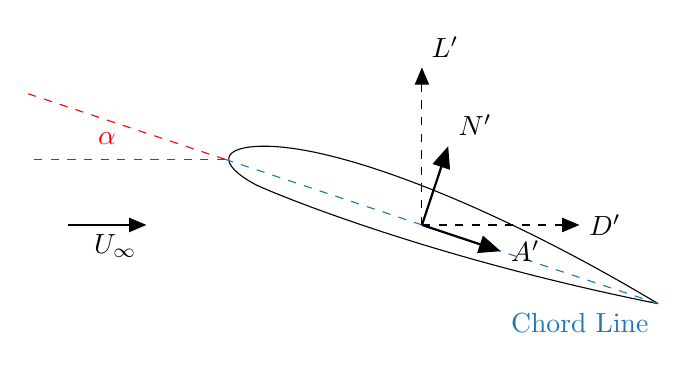
\begin{tikzpicture}
        \draw[rounded corners = 1cm] (6,-2)  .. controls (4, -0.8) and (2,0)  .. (0, 0) .. controls (1, -0.55) and (3, -1.4) .. (6,-2);
        \draw[dashed, blue] (0.5,-0.1666) -- (6,-2) node[anchor=north east] {Chord Line};
        \draw[dashed, red] (0.5,-0.1666) -- (-2,0.666);
        \draw[dashed, red] (0.5,-0.1666) -- (-2, -0.1666);
        \draw[red] (-1, 0.1) node {$\alpha$};
        \draw[->] (-1.5,-1) -- (-0.5,-1) node[anchor=north east] {$U_\infty$};
        \draw[thick,->] (3, -1) -- (3.3333, 0) node[anchor=south west] {$N'$};
        \draw[thick,->] (3, -1) -- (4, -1.333) node[anchor=west] {$A'$};
        \draw[dashed, ->] (3, -1) -- (3, 1) node[anchor=south west] {$L'$};
        \draw[dashed, ->] (3, -1) -- (5, -1) node[anchor=west] {$D'$};
    \end{tikzpicture}
    \caption{Definition of variables related to forces on an airfoil}
    \label{fig:airfoil_directions}
\end{figure}

Lift, drag, and moment are nondimensionalized using Equations \ref{eq:cl}, \ref{eq:cd}, and \ref{eq:cm} respectively where\\
$q_\infty\equiv\frac{1}{2}\rho_\infty U_\infty^2$ is the freestream dynamic pressure and $C$ is the chord length.

\begin{align}
    C_L &= \frac{L'}{q_\infty C}
    \label{eq:cl}\\
    C_D &= \frac{D'}{q_\infty C}
    \label{eq:cd}\\
    C_M &= \frac{M'}{q_\infty C^2}
    \label{eq:cm}
\end{align}

\subsection{Stall}
Airfoil stall is characterized by a significant separation in flow from the airfoil surface resulting in loss of lift, increased drag, and a zero-or-positive pitching moment. Such conditions lead to unpredictable behaviour of an airfoil, and reduced aircraft controlability due to reduced effectiveness of aircrat control surfaces. It is important to understand the behaviour of a varying the angle of attack on the lift, drag, and moment characteristics of an airfoil to understand the limitations of the airfoil.

% -----------------------------------------------------------------------------
%   Experimental Set-Up
% -----------------------------------------------------------------------------


\section{Experimental Set-Up}

This details the lab setup and experimental procedure used in the experiment.

\subsection{Apparatus}
The Clark Y airfoil is 3D printed, with 19 small holes along the centerline of the span allowing pressure measurements over the surface. Pressure tap locations are presented in Table \ref{tab:pressure_taps}.

\begin{table}
    \centering
    \begin{tabular}{|c||c|c|c|c|c|c|c|c|c|c|}\hline
        x/c & 0 & 0.03 & 0.06 & 0.10 & 0.15 & 0.20 & 0.30 & 0.40 & 0.55 & 0.70 \\\hline
        Tap Number & 1 & 2 & 3 & 4 & 5 & 6 & 7 & 8 & 9 & 10\\\hline \hline
        x/c & 0.85 & 1.00 & 0.90 & 0.60 & 0.40 & 0.30 & 0.20 & 0.10 & 0.05&\\\hline
        Tap Number & 11 & 12 & 13 & 14 & 15 & 16 & 17 & 18 & 19&\\\hline
    \end{tabular}
    \caption{Static pressure tap locations for the test model. Taps 1 through 12 are on the top surface, while 13 thought 19 are on the bottom surface.}
    \label{tab:pressure_taps}
\end{table}

Tests are conducted in an ELD Model 402B subsonic open-return wind tunnel, with a 304.8 x 304.8 x 610 mm  square prismatic test section. The airfoil is shown installed in Figure \ref{fig:wind_tunnel_setup}. The airfoil is installed using a rotary mechanism to vary the angle of attack across runs, shown in Figure \ref{fig:aoa_select}.

\begin{figure}
    \centering
    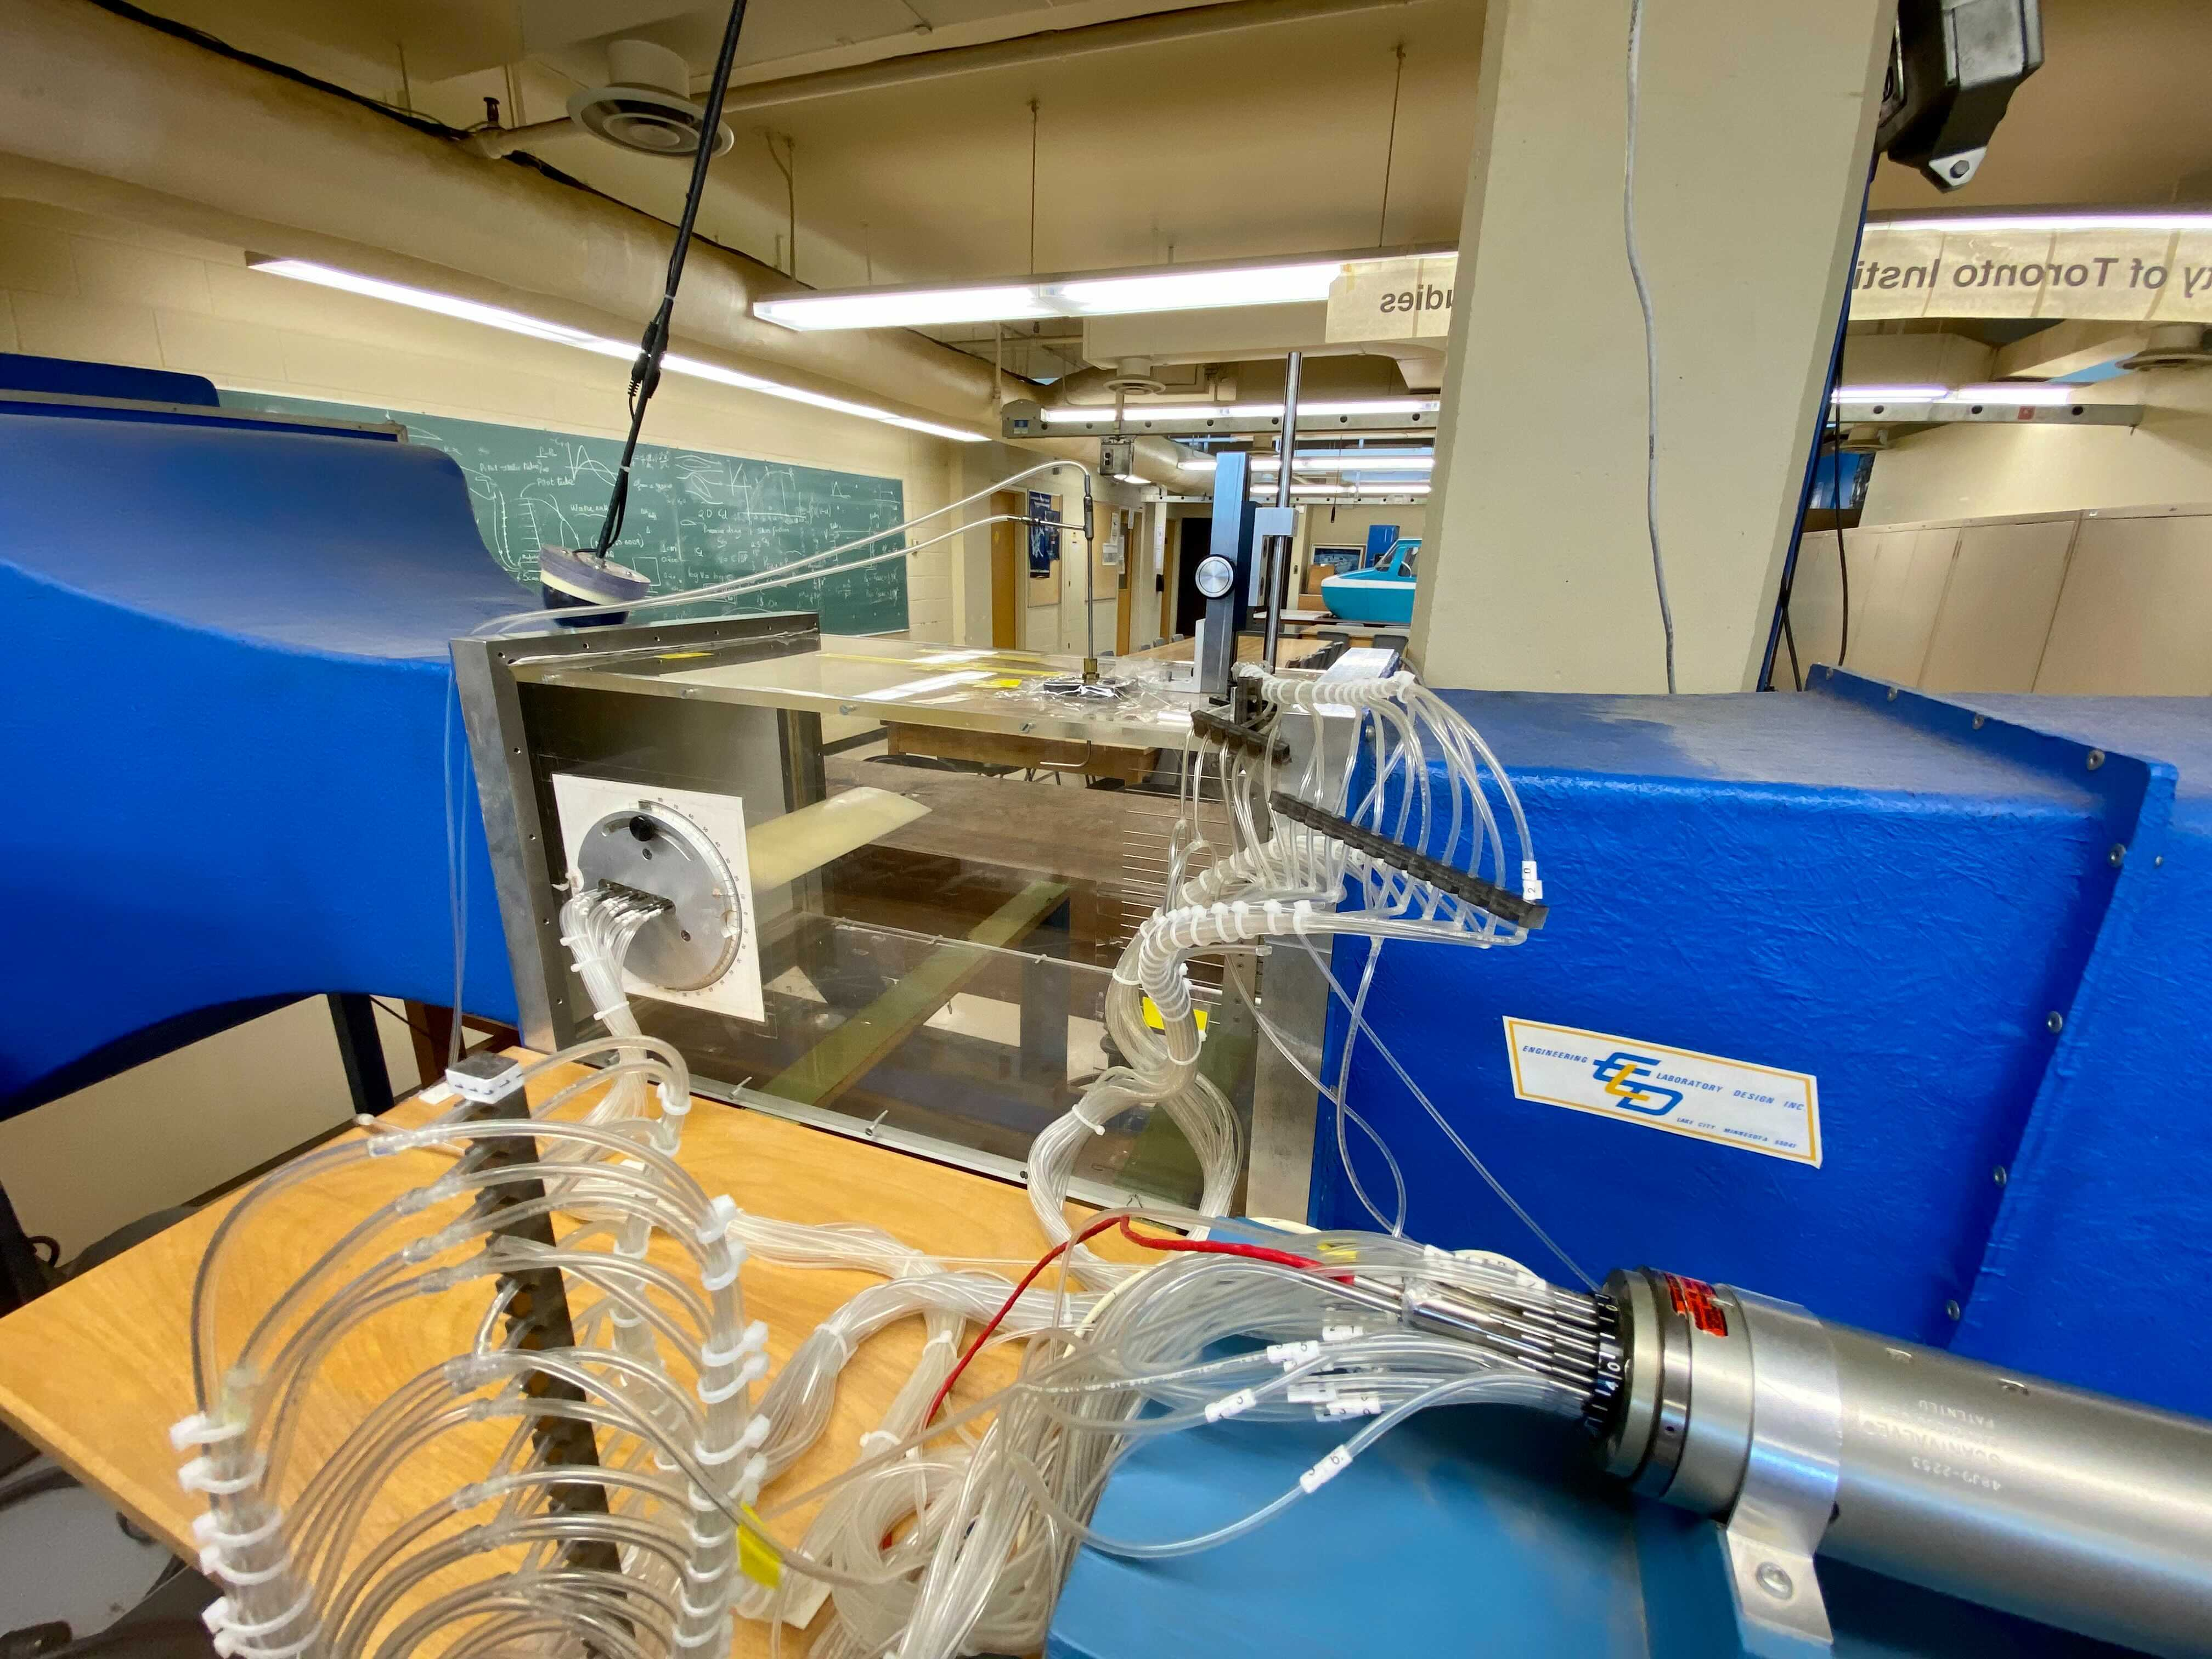
\includegraphics[width=0.6\textwidth]{Apparatus Pictures/wind_tunnel_setup.jpg}
    \caption{The wind tunnel section, with the 3D printed test model installed.}
    \label{fig:wind_tunnel_setup}
\end{figure}

\begin{figure}
    \centering
    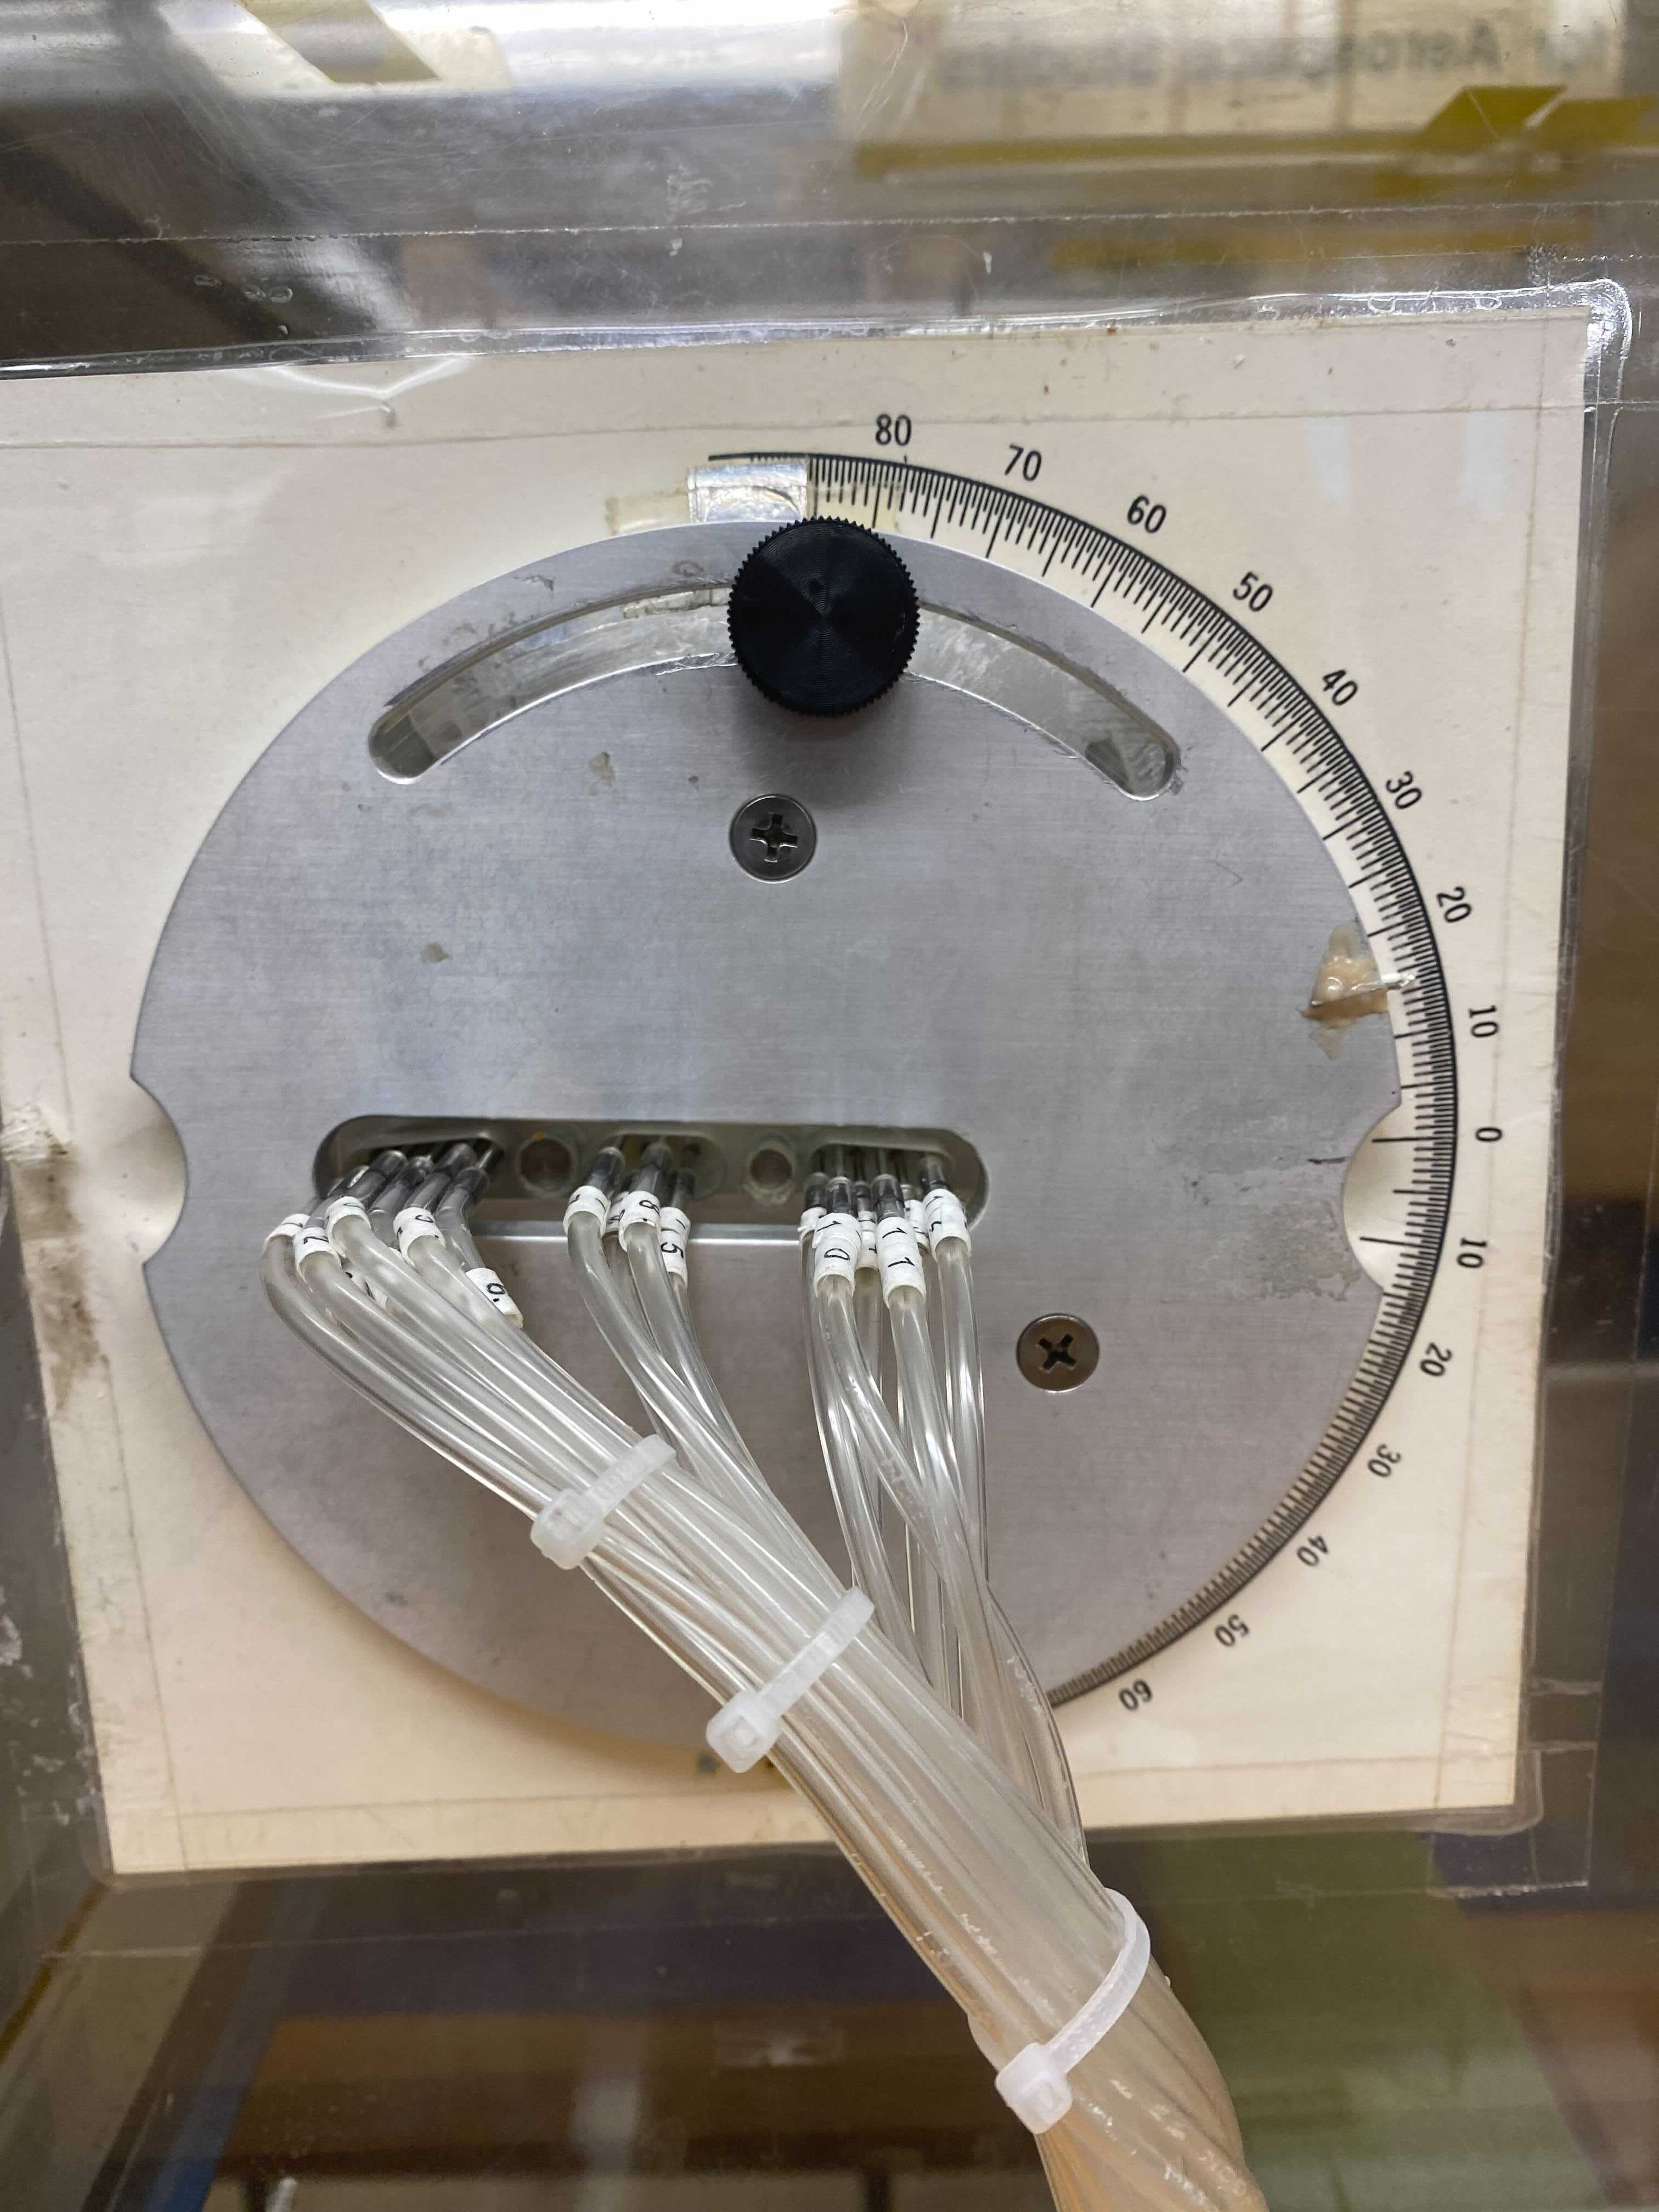
\includegraphics[width=0.4\textwidth]{Apparatus Pictures/aoa_selector.jpg}
    \caption{Adjustable rotary mechanism to hold the airfoil at different angles of attack.}
    \label{fig:aoa_select}
\end{figure}

In addition to 19 static pressure taps on the airfoil, there are 17 pitot tubes arranged as a rake, placed 27 cm downstream of the airfoil's trailing edge. A pitot-static tube placed upstream of the airfoil is used for wind tunnel speed measurement, with the pitot tube connected to a Betz manometer, and the static tube used as the reference pressure in the two measurement devices.

A total of 38 pressure tubes exit the wind tunnel; one is the upstream pitot tube connects to the Betz manometer, and the other 37 connect to the measurement devices. The latter 37 tubes are bifurcated to feed into a multi-channel Scanivalve-transducer system, and the other into an inclined manometer.

The Scanivalve system is pictured in Figure \ref{fig:scanivalve}. An analog pressure transducer is connected to the sampling and reference outputs of the Scanivalve. The connected sampling tube rapidly switches between 36 pressure tubes such that the pressure transducer measures the pressure difference between the sampled pressure and the reference pressure from the upstream static tube. The analog signal from the pressure transducer is fed into a data acquisition card, connected to a computer running MATLAB to collect data.

\begin{figure}[h]
    \centering
    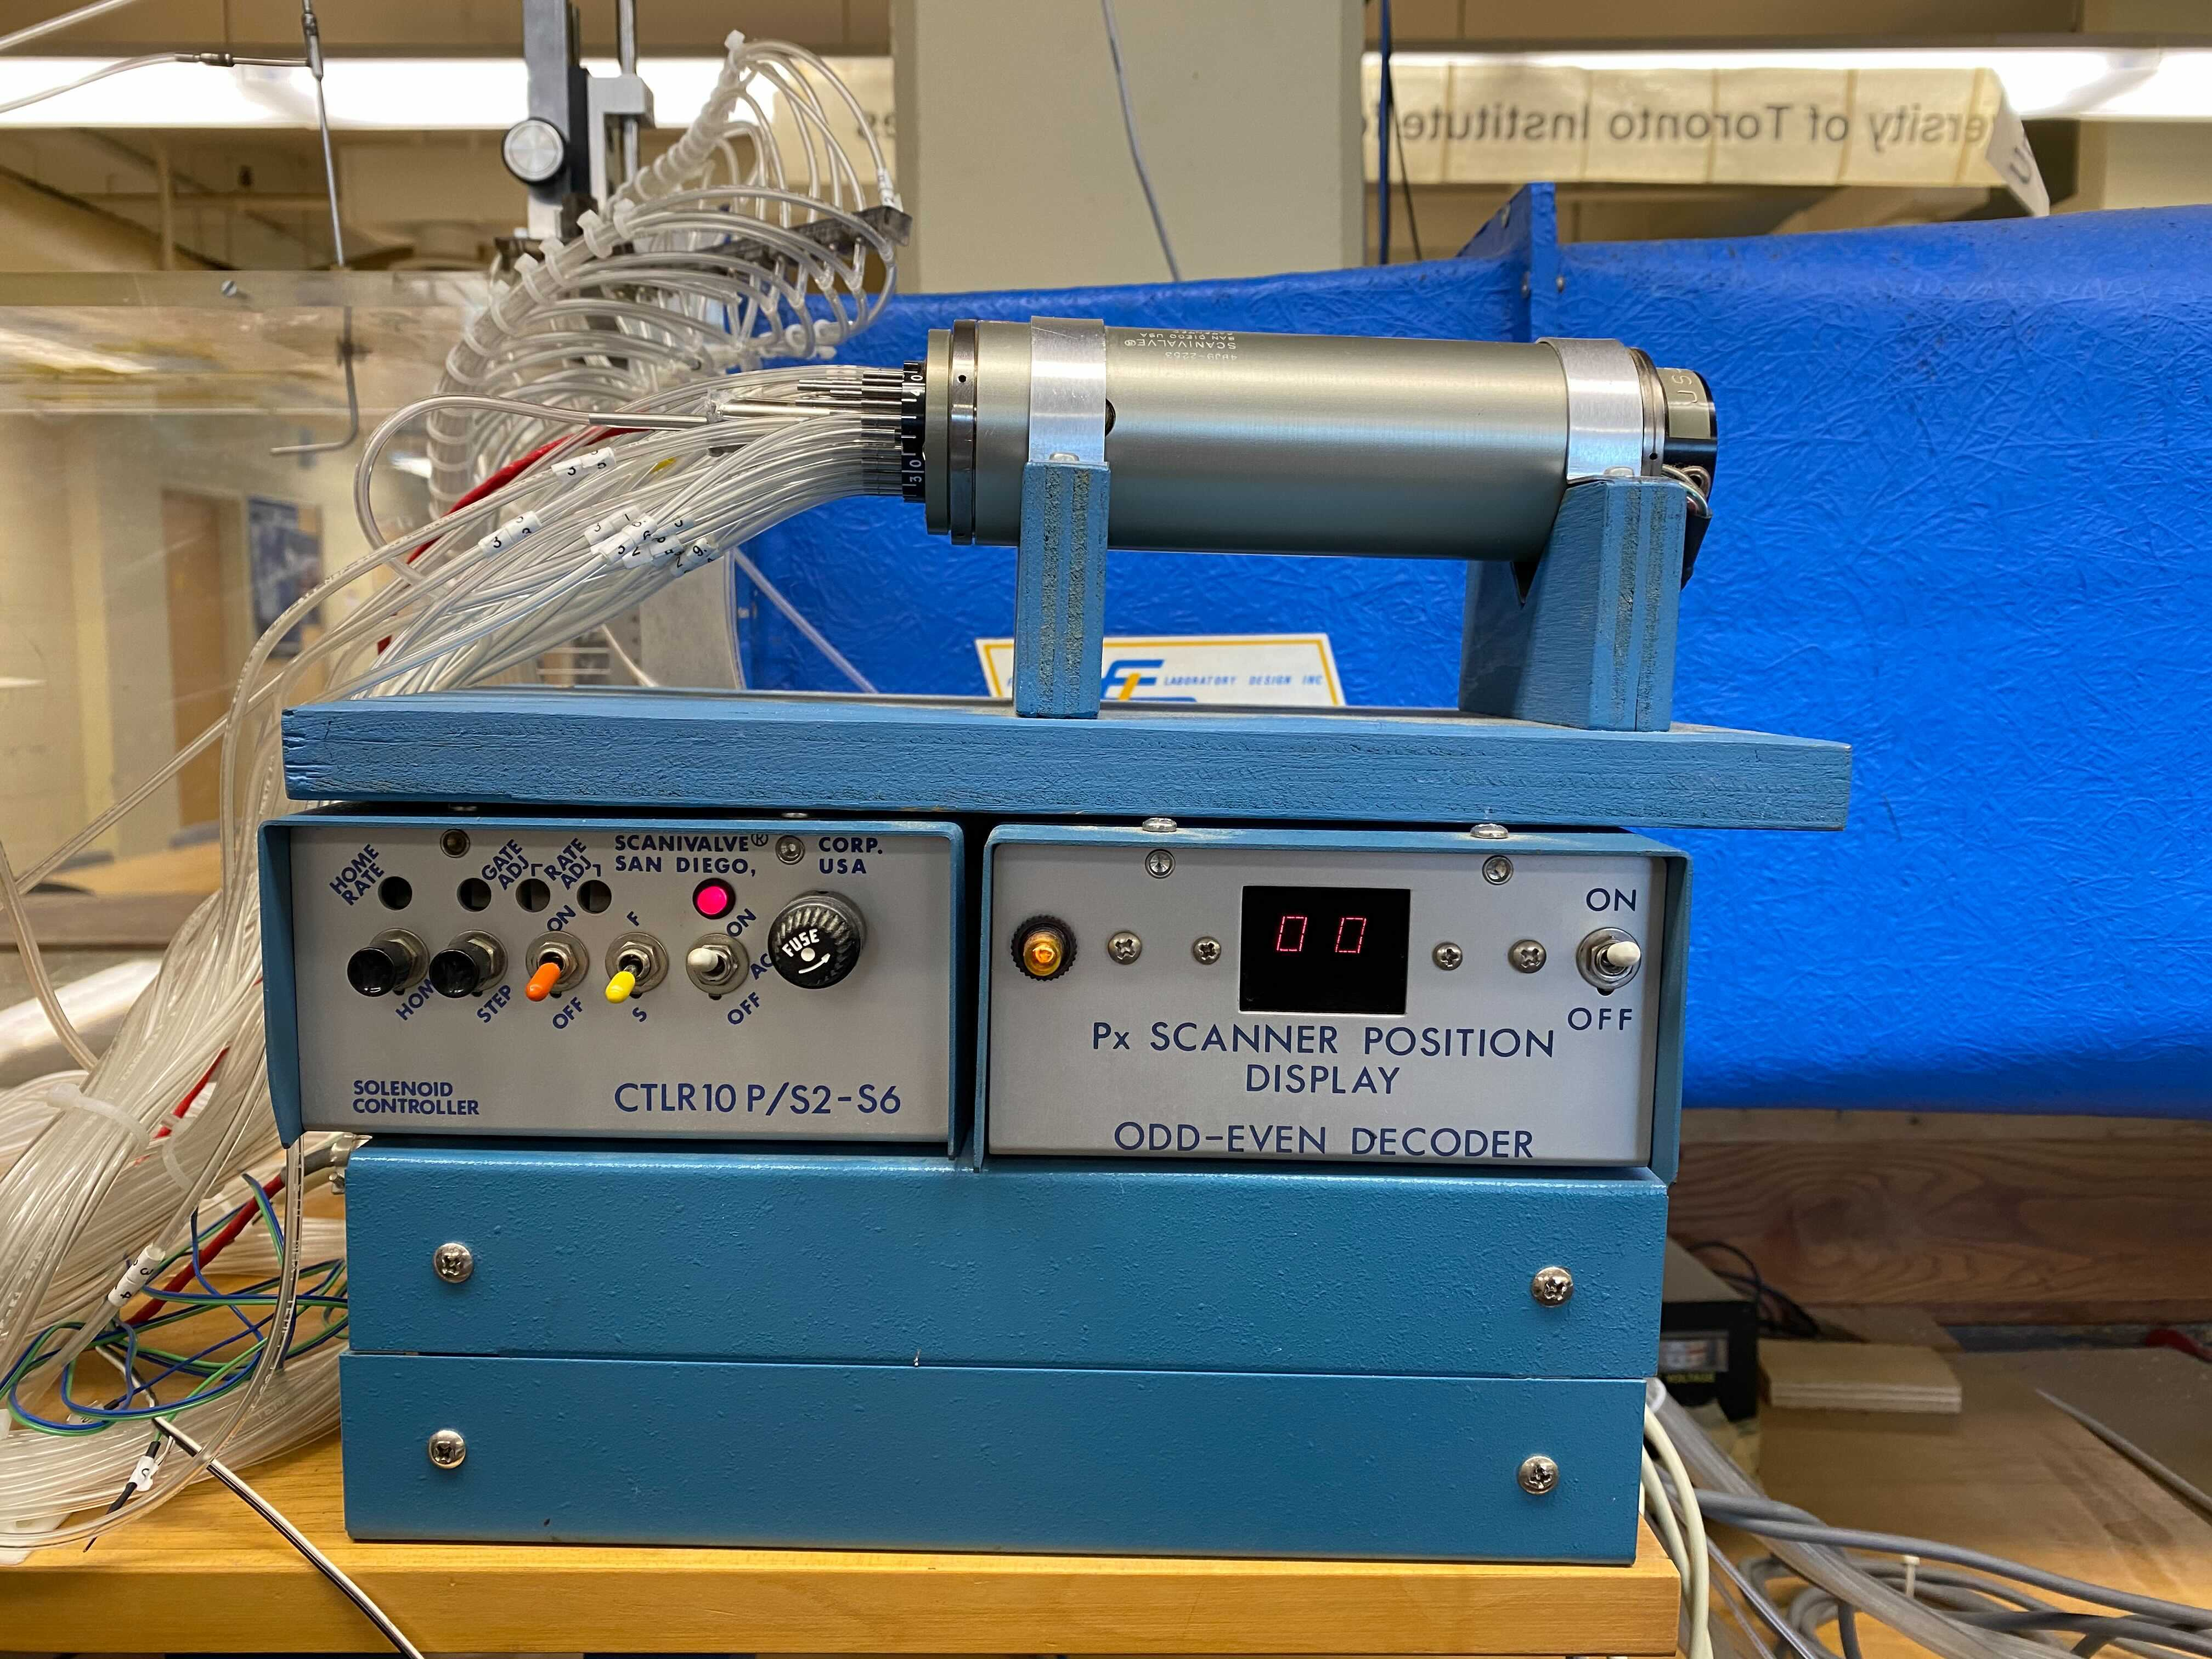
\includegraphics[width=0.4\textwidth]{Apparatus Pictures/scanivalve.jpg}
    \caption{Scanivalve system, connected to a pressure transcuder. The system allows rapid switching of each of the 36 channels to the transducer to sweep through all pressure measurements.}
    \label{fig:scanivalve}
\end{figure}

The inclined manometer takes in 36 input channels and one reference channel to measure the pressure difference between each of the 36 inputs compared to the reference. The reference pressure is set to that of the upstream static tube.

\begin{figure}[h]
    \centering
    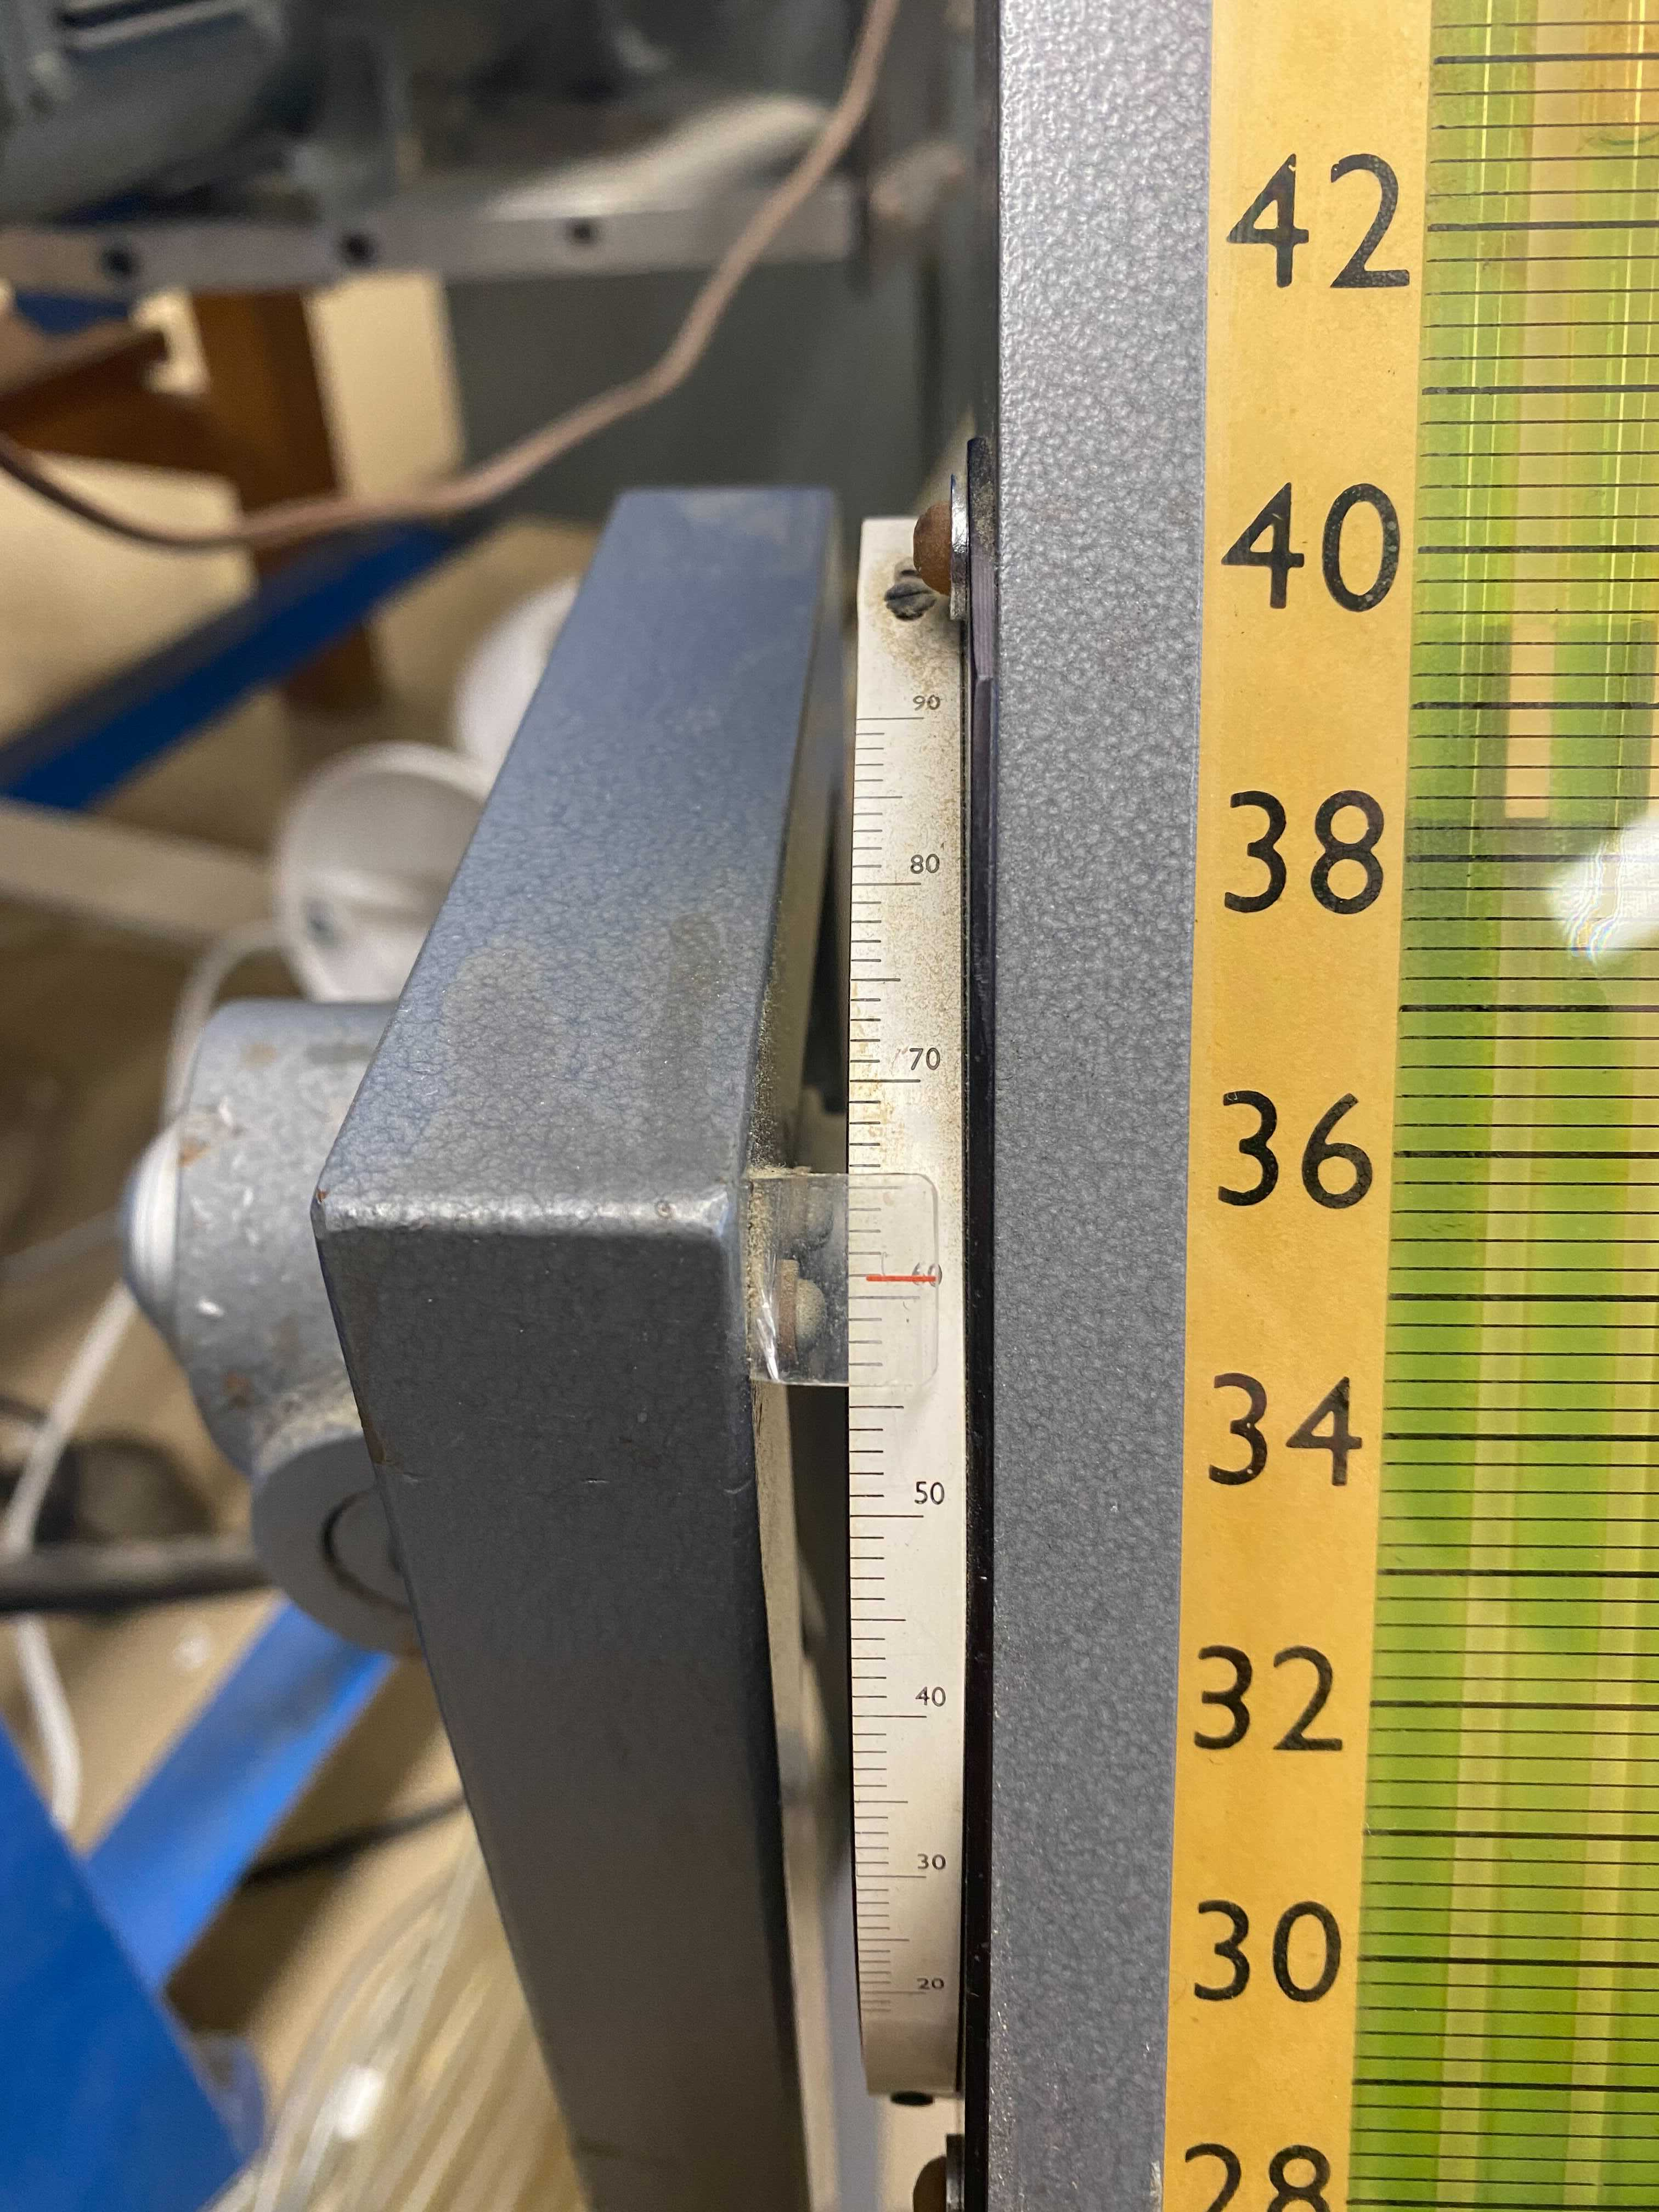
\includegraphics[width=0.4\textwidth]{Apparatus Pictures/inclined_manometer_slope_graduations.jpg}
    \caption{Inclined manometer.}
    \label{fig:manometer}
\end{figure}

\subsection{Procedure}

% What is measured and how it is acquired.

The procedure used for acquisition of pressure measurements is as follows:

\begin{enumerate}

    \item The sample frequency and data acquisition time are determined such that the pressure transducer measurements admit a $\pm 1\%$ accuracy. The wind tunnel is set to a speed of $110\si{km.h^{-1}}$. A series of representative measurements from the pressure transducer output are taken and autocorrelated to determine the sample frequency and data acquisition time required for $\pm 1\%$ accuracy.
    
    \item The calibration curve for the pressure transducer is constructed next. This allows interpolated conversion from voltage-pressure representations of pressure transducer into equivalent pressure values. The curve is constructed by taking ten different voltage-pressure measurements are taken at varying wind tunnel speeds using scanivalve readings while finding the corresponding pressure measurements using the Betz manometer. This correspondence between representations is used to calibrate the pressure-voltage curve of the transducer.
    
    \item The wind tunnel speed is set back to $110\si{km.h^{-1}}$ and wind tunnel's pitot-static pressure difference is measured to calculate the actual wind speed experiences in the wind tunnel.
    
    \item Next, the angle of attack is changed in the positive and negative directions to determine the stall angle values. Using this information, it is determined what angles of attack would be useful to measure to accurately represent the airfoil properties up to and past stall conditions. The angle of attack values chosen were \numlist{0;3;6;8;10;11;13;15;16;17;20} degrees.

    \item Cycling through each angle of attack, the pressure distribution is measured along the top and bottom surfaces of the airfoil in addition to the pressure distribution in the airfoils wake. These values are measured by reading the fluid height changes from the inclined manometer. To get greater precision in the wake measurements, the wake rake is displaced by $5\si{mm}$ for a second round of measurements to fill the gaps between each rake tube. Pressure measurements are taken using two methods: (1) the pressure transducer fed by the scanivalve device and (2) the inclined manometer.

\end{enumerate}

Once the pressure measurements were taken, the data is pre-processed to obtain pressure distributions over the airfoil and in its wake. This pre-processing follows the following procedure depending on the measurement method.

\begin{enumerate}

    \item For data calculated using the pressure transducer, the calibration curve for the pressure transducer is used to convert raw data into equivalent pressure readings, using an interpolation script.

    \item For data calculated using the inclined manometer, the change in static pressure is determined from the change of fluid height for each manometer tube compared to an "at-rest" state which and using Bernoulli's relation.

\end{enumerate}

After the data is pre-processed, the data is analyzed to determine the lift, moment, and drag coefficients as well as a measure of the lift, moment, and pressure drag of the airfoil up to and past the point of stall. The analysis is done using the methods described in section \ref{sec:introduction_and_background}.

%% TODO: mention image analysis process

% -----------------------------------------------------------------------------
%   Results and Discussion
% -----------------------------------------------------------------------------


\section{Results and Discussion}

\subsection{Comparison with XFOIL}
Reference results with XFOIL are obtained from analysis of the .dat file obtained from \href{http://airfoiltools.com/airfoil/details?airfoil=clarky-il}{airfoiltools.com}, using 240 panels nodes in the viscous solver mode at $Re = 200000$. Pressure distributions, and the dimensionless coefficients are determined for all $\alpha$ values used in the experiment. The results as are follows:

\subsection{Comparison with other experiments}
Experimental performance data of a Clark Y airfoil is available in literature
\cite{lyon_broeren_giguere_gopalarathnam_selig_1997}.

% -----------------------------------------------------------------------------
%   Conclusion
% -----------------------------------------------------------------------------


\section{Conclusion}


% -----------------------------------------------------------------------------
%   Bibliography
% -----------------------------------------------------------------------------


\bibliographystyle{ieeetr}
\bibliography{biblio}


% -----------------------------------------------------------------------------
%   Appendix
% -----------------------------------------------------------------------------


\appendix
\section{Pressure Measurements}
\subsection{Scanivalve Measurements}
NOTE: These tables are not final; just here to test.
\begin{table}
    \centering
    \begin{tabular}{|c|c|c|c|c|c|c|c|c|c|c|c|c|c|c|c|c|c|c|c|}\hline
         $\alpha$ & \multicolumn{19}{|c|}{Airfoil Ports ($\num{1e3}\si{V}$)} \\\hline
         \ang{0} & 519 & -1 & -176 & -229 & -306 & -341 & -297 & -261 & -232 & -178 & -48 & 70 & 73 & 38 & 16 & -16 & -47 & -95 & -152  \\\hline
         \ang{3} & 439 & -319 & -449 & -457 & -459 & -471 & -389 & -339 & -291 & -153 & -49 & 82 & 94 & 83 & 89 & 78 & 67 & 70 & 95 \\\hline
         \ang{6} & -52 & -711 & -744 & -685 & -661 & -622 & -518 & -436 & -306 & -182 & -62 & 75 & 107 & 126 & 143 & 146 & 161 & 205 & 274\\\hline
    \end{tabular}
    \caption{Caption}
    \label{tab:pressure_scanivalve}
\end{table}

\begin{table}
    \centering
    \begin{tabular}{|c|c|c|c|c|c|c|c|c|c|c|c|c|c|c|c|c|c|}\hline
         $\alpha$ & \multicolumn{17}{|c|}{Rake Ports 1 ($\num{1e3}\si{V}$)} \\\hline
         \ang{0} & 544 & 533 & 530 & 522 & 521 & 522 & 521 & 520 & 519 & 459 & 509 & 521 & 519 & 521 & 552 & 508 & 528  \\\hline
         \ang{3} & 547 & 551 & 543 & 529 & 534 & 529 & 533 & 539 & 534 & 504 & 482 & 525 & 528 & 534 & 565 & 542 & 535 \\ \hline
    \end{tabular}
    \caption{RAW}
    \label{tab:pressure_rake1}
\end{table}

\begin{table}
    \centering
    \begin{tabular}{|c|c|c|c|c|c|c|c|c|c|c|c|c|c|c|c|c|c|}\hline
         $\alpha$ & \multicolumn{17}{|c|}{Rake Ports 2 ($\num{1e3}\si{V}$)} \\\hline
         \ang{0} &  545 & 534 & 530 & 532 & 536 & 530 & 511 & 529 & 508 & 469 & 523 & 527 & 528 & 530 & 557 & 533 & 534   \\\hline
        \ang{3} & 549 & 544 & 548 & 533 & 536 & 532 & 533 & 526 & 537 & 479 & 515 & 536 & 517 & 550 & 564 & 548 & 528 \\\hline
    \end{tabular}
    \caption{Caption}
    \label{tab:pressure_rake2}
\end{table}

\subsection{Manometer Measurements}

\appendix
\section{Uncertainty Propagation}
\subsection{Manometer Pressure}
Reference height $h_R = 18.2 \ \si{cm}$ (assumed errorless) on manometer used for baseline. $\theta = 61 \pm 0.1^\circ$
\begin{align*}
    P_{mano} &= -\rho g (h - h_R) \sin\theta\\
    \delta P_{mano} &= \sqrt{\left(-\rho g \sin \theta \delta h\right)^2 + \left(-\rho g  (h-h_R)\cos\theta \delta \theta\right)^2}\\
    \delta P_{mano} &= \sqrt{\left(-\rho g \sin \theta \delta h\right)^2 + \left(\frac{P_{mano}}{\tan \theta}\right)^2}
\end{align*}

\subsection{Flow Velocity}
For cases where we want the velocity of airfoil at a single pitot tube.
\begin{align*}
    U_\infty &=  \sqrt{\frac{2 P}{\rho}} \\
    \delta U_\infty &= \frac{P}{U_\infty \rho}
\end{align*}

\subsection{Free Stream Velocity}
An average free stream velocity was obtained using ports 20 and 36. Assume zero error in $\rho$.
\begin{align*}
    U_\infty &= \frac{1}{2} \left(\sqrt{\frac{2 P_{20}}{\rho}} + \sqrt{\frac{2 P_{36}}{\rho}} \right) \\
    \delta U_\infty &= \sqrt{\left(\frac{1}{2U_\infty \rho} \delta P_{20}\right)^2 + \left(\frac{1}{2U_\infty \rho } \delta P_{36}\right)^2}
\end{align*}

\subsection{Velocity Deficit}
This is used to create the wake velocity distribution.
\begin{align*}
    \Delta V &= U_\infty - u\\
    \delta \Delta V &= \sqrt{\delta U_\infty^2 + \delta u^2}
\end{align*}

\subsection{Drag Force}
This was evaluated numerically using trapezoidal rule, ignoring the errors associated with it.
\begin{align*}
    D &= \rho\int u (U_\infty - u) dS\\
    \diffp{D}{{U_\infty}} &= \rho \int  u dS\\
    \diffp{D}{u} &= \rho \int (U_\infty - 2u) dS\\
    \delta D &= \sqrt{\left(\rho \int  u dS \ \delta U_\infty \right)^2 + \left(\rho \int (U_\infty - 2u) dS \ \delta u \right)^2}
\end{align*}

\subsection{Dynamic Pressure}
\begin{align*}
    q &= \frac{1}{2} \rho u^2\\
    \delta q &= \rho u
\end{align*}

\subsection{Drag Coefficient}
Assume the chord length to be known perfectly.
\begin{align*}
    c_D &= \frac{D}{q_\infty c}\\
    \delta c_D &= \sqrt{\left(\frac{\delta D}{q_\infty c}\right)^2 + \left( \frac{\delta q c_D}{q} \right)^2}
\end{align*}

\end{document}
